\documentclass[a4paper,12pt]{article}

\usepackage[margin=2.5cm]{geometry}
\usepackage{fontspec}
\usepackage{polyglossia}
\setdefaultlanguage{bulgarian}
\setotherlanguage{english}
\setmainfont{Times New Roman}
\usepackage{graphicx}
\usepackage{booktabs}
\usepackage{amsmath}
\usepackage{caption}
\usepackage[hidelinks]{hyperref}
\usepackage{parskip}
\usepackage{float}
\setlength{\parindent}{1.25cm}

\captionsetup{font=small, labelfont=bf}

\title{Проверка на съответствие на потребителски интерфейс с толерантност към малки измествания}
\author{Алекс Цветанов\\
фак. № 121326006, група 221а\\
e-mail: ...}
\date{}

\begin{document}

\maketitle

\begin{abstract}
\noindent\textbf{Резюме.}
При всяка промяна в продукцията трябва да се провери, че потребителският интерфейс все още съответства на желания интерфейс – дизайн във Figma или одобрена реализация. Пикселно-точното сравнение не работи добре за тази задача: изместване на целия екран с 1–4 пиксела не променя потребителското изживяване, но предизвиква фалшиви тревоги, а чернови от дизайн рядко съвпадат пиксел по пиксел. Предлагаме многослойна проверка, която комбинира класически методи за обработка на изображения, замразени предобучени характеристики и малка конволюционна невронна мрежа, и връща вердикт SAME, MINOR или DIFFERENT. Оценяваме слоевете върху 1412 статични двойки от четири платформи и две теми, от които 204 са проверени от човек, а останалите 1208 са съгласувани между два AI прегледа без човешка проверка. На всички двойки логистичният стекинг достига AUC 0.94 (95\% доверителен интервал 0.92–0.95), а отделните най-добри слоеве са DINOv2 и ResNet-18 с топ-5 плочки (0.92 и 0.89). Върху 204-те спорни двойки обаче същите слоеве падат до около 0.53, а GMSD (0.76) и хамфър разстоянието по контури (0.74) са по-добри. Това показва, че високите резултати на всички двойки се дължат основно на лесните съгласувани двойки. При изместване с 4 пиксела пикселният SSIM маркира 82\% от двойките, които трябва да са SAME, докато LBP маркира 44\%, а ResNet-18 с топ-5 плочки – 33\%. Обучената конволюционна мрежа е на ниво 0.85 върху всички двойки, но без предварително обучение върху нашите етикети; за GIF файловете нито един слой не разделя четирите положителни двойки надеждно.
\end{abstract}

\noindent\textbf{Ключови думи:} проверка на интерфейс; толерантност към измествания; SSIM; LBP; ResNet; DINOv2; откриване на промени; GIF.

\section{Въведение}
Потребителският интерфейс се променя при всяка промяна в продукцията. Желаният интерфейс обикновено е дизайн във Figma или одобрена реализация, а текущата разработка е онова, което се изпраща на потребителите. Задачата е да се провери програмно, че всяка промяна не нарушава желания интерфейс. Пикселно-точното сравнение е първата идея, но тя не работи добре: черновите от дизайн рядко съвпадат пиксел по пиксел, а незначителни промени – като изместване на целия екран с 1–4 пиксела – не променят потребителското изживяване, но водят до фалшиви тревоги. Затова проверката трябва да е толерантна към дребни отклонения и да улавя промени в структурата, текста и взаимното разположение на елементите.

Задачата е свързана с няколко теми от курса по компютърно зрение: филтрация и оценка на качеството на изображения, откриване на контури, сегментация, текстурен анализ, съпоставяне на ключови точки и разпознаване с машинно обучение и дълбоко обучение. В работата сравняваме 14 подхода върху 1412 статични двойки (етикетите са съгласувани между Claude и Gemini, а 204 спорни случая са проверени от човек) и 34 GIF двойки с човешки етикети. Към класическите методи добавяме замразени предобучени характеристики и малка конволюционна мрежа, обучена върху синтетични промени, за да проверим дали обучението помага. Освен точността измерваме и устойчивостта на всеки слой към изместване на екрана с 0–4 пиксела.

Във всички раздели ни интересуват две страни. Желаният интерфейс е референцията, а текущата разработка е кандидатът. Етикетът SAME означава, че потребителското изживяване съвпада, а DIFFERENT – че е нарушено. В раздел~\ref{sec:methods} описваме подходите и протокола, в раздел~\ref{sec:results} – резултатите, в раздел~\ref{sec:shift} – устойчивостта към изместване, а в раздел~\ref{sec:discussion} анализираме грешките и посочваме следващите стъпки. Ако не е указано друго, всички AUC стойности са с 95\% доверителен интервал, получен с bootstrap от 2000 повторения~\cite{efron1993}. AUC е мярката за качеството на подреждането~\cite{hanley1982}.

\section{Методи}\label{sec:methods}

\subsection{Данни и протокол}
Данните са получени при портиране на MAUI приложение към C++. Еталонното MAUI приложение играе ролята на желан интерфейс, а C++ портът – на развиваща се реализация. Това е модел на проблема, а не самият случай. Снимките са заснети на четири платформи (Android, iOS, Mac Catalyst, Windows) в светла и тъмна тема и образуват 1412 статични двойки.

Всяка двойка има окончателен етикет ACCEPTED или DECLINED. Двойка, за която двата AI прегледа (Gemini и Claude Opus) дават различен вердикт, е проверена от човек: 204 двойки, от които 175 DECLINED и 29 ACCEPTED. Останалите 1208 двойки имат съгласувания вердикт на двата прегледа без човешка проверка; тези етикети са по-малко надеждни, защото всички AI прегледи са работили върху същите изображения. Общо има 1157 ACCEPTED и 255 DECLINED. GIF набора има 34 двойки, от които 4 DIFFERENT.

Оценяваме AUC върху всички двойки, върху съгласуваните и върху проверените от човек двойки отделно. Доверителните интервали са bootstrap с 2000 повторения~\cite{efron1993}. Стекингът се оценява с 5-кратна стратифицирана кръстосана валидация.

\subsection{Класически слоеве}
Всички слоеве връщат оценка, по-голяма при по-голяма разлика. Първият е SSIM по плочки~\cite{wang2004}: изображението се дели на мрежа $16\times16$, а оценката е най-лошата плочка, $s_{\text{SSIM}} = \max_t (1 - \overline{\text{SSIM}}_t)$.

GMSD~\cite{xue2014} сравнява големините на градиентите, получени с оператора на Prewitt, и измерва разсейването на сходството:
\begin{equation}\label{eq:gmsd}
\text{GMS}(x) = \frac{2 m_a(x) m_b(x) + c}{m_a(x)^2 + m_b(x)^2 + c}, \qquad s_{\text{GMSD}} = \sigma_x\bigl(\text{GMS}(x)\bigr),
\end{equation}
където $m_a$ и $m_b$ са големините на градиентите на двете изображения, $c = 170$, а $\sigma_x$ е стандартното отклонение по всички пиксели.

Контурите се извличат с детектора на Canny~\cite{canny1986}. Симетричното хамфър разстояние~\cite{borgefors1988} е
\begin{equation}\label{eq:chamfer}
s_{\text{хамфър}} = \frac{1}{2D}\Bigl(\overline{d_A(E_B)} + \overline{d_B(E_A)}\Bigr),
\end{equation}
където $E_A$ и $E_B$ са контурните пиксели на двете изображения, $d_A$ е разстоянието до най-близкия контурен пиксел на $A$, а $D$ е диагоналът на изображението.

Цветовата оценка сравнява RGB хистограми с 4 интервала на канал по плочки: $s_{\text{цвят}} = \max_t H(p_t, q_t)$, където $H(p,q) = \sqrt{1 - \sum_i \sqrt{p_i q_i}}$ е разстоянието на Хелингер.

Текстурата се описва с равномерни LBP кодове~\cite{ojala2002} с $P=8$, $R=1$ и хистограма от 10 интервала по плочки. Оценката е $\max_t \chi^2(h_t^A, h_t^B)$ с $\chi^2(h,g) = \tfrac12 \sum_i (h_i - g_i)^2 / (h_i + g_i + \varepsilon)$.

ORB ключови точки~\cite{rublee2011} се съпоставят с праг 0.75 за отношението на разстоянията, след това се оценява хомография с RANSAC~\cite{fischler1981} и праг 4 пиксела. Оценката е $1 - n_{\text{инл}} / \min(n_A, n_B)$.

Сегментацията използва k-means ($k=6$) върху общата палитра на двете изображения, след което свързаните компоненти на всеки цвят се съпоставят по припокриване на обхващащите правоъгълници (IoU $\ge 0.5$). Оценката е делът на несъпоставената площ.

\subsection{Замразени предобучени характеристики}
Използваме ResNet-18~\cite{he2016} (слой 3, вход $512\times512$) и DINOv2 ViT-S/14~\cite{oquab2024} (вход $448\times448$), като теглата са замразени. Характеристиките се осредняват до мрежа $16\times16$, за всяка плочка се изчислява косинусово разстояние $d_t = 1 - \cos(f_t^A, f_t^B)$, а оценката е максимумът или средната стойност на петте най-лоши плочки.

\subsection{Обучена конволюционна мрежа}
Мрежата е с ранно сливане (early fusion), по идея на FC-EF~\cite{daudt2018}, с кодер-декодер структура като U-Net~\cite{ronneberger2015}. Входът са двете изображения, подредени в 6 канала, а изходът е логит на промяната за всеки пиксел. Мрежата има 16 канала в първия слой, 32 в средния и около 31 хиляди параметъра.

Синтетичните данни се получават от MAUI еталонни снимки, които не се използват в етикетите. Вземат се 1200 участъка $256\times256$ и за всеки участък се създава отрицателна или положителна двойка. Отрицателните примери са фотометрично изменени изображения (яркост, шум и цветово отместване с до 6 нива). Положителните примери съдържат от 1 до 3 промени: запълване на правоъгълник, инверсия, изместване на област с 2–12 пиксела, копиране от друго място или линии с размер на текст. Загубата е двоична кръстосана ентропия с тегло 3 за положителните примери плюс загуба на Dice; оптимизаторът е Adam~\cite{kingma2015} с косинусово намаляване на скоростта на обучение, 2000 стъпки и партида от 32 участъка $128\times128$.

Оценката на двойка е максимумът по прозорци $128\times128$ със стъпка 96 от средната вероятност на блокове $8\times8$. Дообучаването използва слаб надзор (multiple-instance learning): имаме само един етикет за цялото изображение, затова загубата е $-y \log s - (1-y)\log(1-s)$ върху максималния прозорец. Дообучаването се провежда с 4-кратна стратифицирана кръстосана валидация.

\subsection{Стекинг и GIF слоеве}
Стекингът е логистична регресия върху 12-те статични оценки, нормализирани по средна стойност и дисперсия, с претегляне на класовете:
\begin{equation}\label{eq:stack}
p(y=1 \mid x) = \sigma\bigl(w^\top x + b\bigr).
\end{equation}
За GIF файловете сравняваме DTW разстоянието върху SSIM стойности~\cite{berndt1994}, хамфър-подобна оценка върху матрицата на разходите на DTW, най-лошия кадър по SSIM и мрежата, приложена върху извадка от 6 кадъра на всяка страна (максимин по кадрите).

\section{Резултати}\label{sec:results}

Таблица~\ref{tab:static} показва AUC за всяка оценка върху трите подмножества. Колоната 1412 е върху всички двойки; колоната консенсус е върху 1208-те съгласувани двойки, а колоната човешки е върху 204-те спорни двойки, проверени от човек.

\begin{table}[H]
\centering
\caption{AUC по слоеве върху всички 1412 двойки, върху съгласуваните 1208 двойки и върху 204-те спорни двойки, проверени от човек (доверителен интервал 95\%).}\label{tab:static}
\scriptsize
\begin{tabular}{lccc}
\hline
Метод & AUC (1412) & AUC (консенсус, 1208) & AUC (човешки, 204) \\
\hline
SSIM по плочки (базова) & 0.811 [0.78, 0.84] & 0.857 [0.82, 0.90] & 0.428 [0.33, 0.52] \\
GMSD & 0.872 [0.85, 0.89] & 0.942 [0.92, 0.96] & 0.763 [0.66, 0.86] \\
Chamfer по контури & 0.814 [0.79, 0.84] & 0.905 [0.88, 0.93] & 0.742 [0.64, 0.83] \\
Цветови хистограми & 0.805 [0.78, 0.83] & 0.859 [0.82, 0.89] & 0.328 [0.22, 0.44] \\
LBP текстура & 0.831 [0.80, 0.86] & 0.931 [0.91, 0.95] & 0.687 [0.60, 0.77] \\
ORB + RANSAC & 0.818 [0.79, 0.84] & 0.894 [0.86, 0.92] & 0.568 [0.46, 0.67] \\
Сегменти (k-means) & 0.673 [0.64, 0.70] & 0.717 [0.66, 0.77] & 0.452 [0.35, 0.55] \\
ResNet-18 плочки (max) & 0.877 [0.86, 0.90] & 0.943 [0.92, 0.96] & 0.507 [0.41, 0.62] \\
ResNet-18 плочки (топ-5) & 0.891 [0.87, 0.91] & 0.958 [0.93, 0.98] & 0.519 [0.42, 0.63] \\
DINOv2 плочки (max) & 0.902 [0.88, 0.92] & 0.959 [0.94, 0.98] & 0.532 [0.43, 0.64] \\
DINOv2 плочки (топ-5) & 0.917 [0.90, 0.93] & 0.964 [0.94, 0.98] & 0.529 [0.43, 0.64] \\
CNN, обучен синтетично & 0.845 [0.82, 0.87] & 0.896 [0.87, 0.92] & 0.427 [0.33, 0.54] \\
Логистичен стекинг (5-кратно CV) & 0.938 [0.92, 0.95] & 0.984 [0.97, 0.99] & 0.676 [0.56, 0.78] \\
\hline
\end{tabular}

\end{table}

На всички двойки стекингът дава AUC 0.938 (0.92–0.95), а DINOv2 с топ-5 плочки е най-добрият отделен слоят с 0.917 (0.90–0.93). ResNet-18 и DINOv2 са на същото ниво на съгласуваните двойки (0.96), но върху спорните двойки падат до около 0.53. Това е главният резултат от оценката: дълбоките плочкови признаци отговарят на съгласуването между двата AI прегледа, а не на човешката преценка за спорните случаи.

Върху спорните двойки най-добрите слоеве са GMSD (0.763, 0.66–0.86), хамфър по контури (0.742, 0.64–0.83) и LBP текстурата (0.687, 0.60–0.77). Стекингът дава 0.676 (0.56–0.78). Цветовите хистограми (0.328) и SSIM по плочки (0.428) са обърнати на тези двойки, което показва, че пикселните и цветовите различия са основният източник на грешки в спорните случаи.

Обучената конволюционна мрежа достига AUC 0.845 върху всички двойки и 0.896 върху съгласуваните, но 0.427 върху спорните. Нейните дообучени варианти бяха оценени само върху предишния по-малък набор от 108 етикета и не са включени в тази таблица.

Фигура~\ref{fig:roc} показва ROC кривите върху всички 1412 двойки (ляво) и върху 204-те човешки проверени двойки (дясно), където всички слоеве са значително по-слаби. Фигура~\ref{fig:heat} показва пример за картата на промяната на мрежата върху негативна двойка от същия набор.

\begin{figure}[H]
\centering
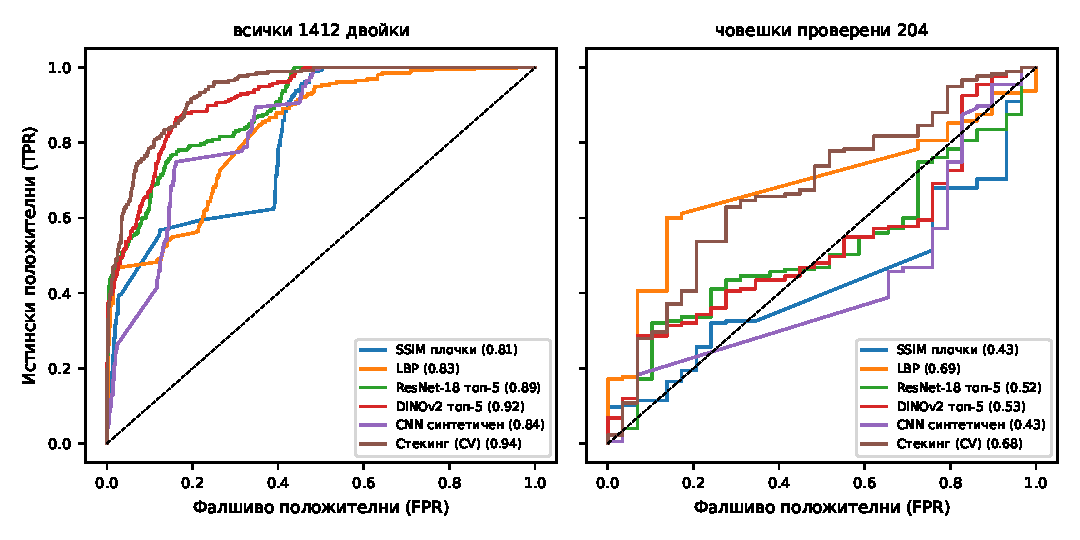
\includegraphics[width=\linewidth]{figures/roc_static.pdf}
\caption{ROC криви върху всички 1412 статични двойки (ляво) и върху 204-те човешки проверени двойки (дясно); AUC е в скоби. Стекингът е оценен с 5-кратно кръстосано валидиране.}\label{fig:roc}
\end{figure}

\begin{figure}[H]
\centering
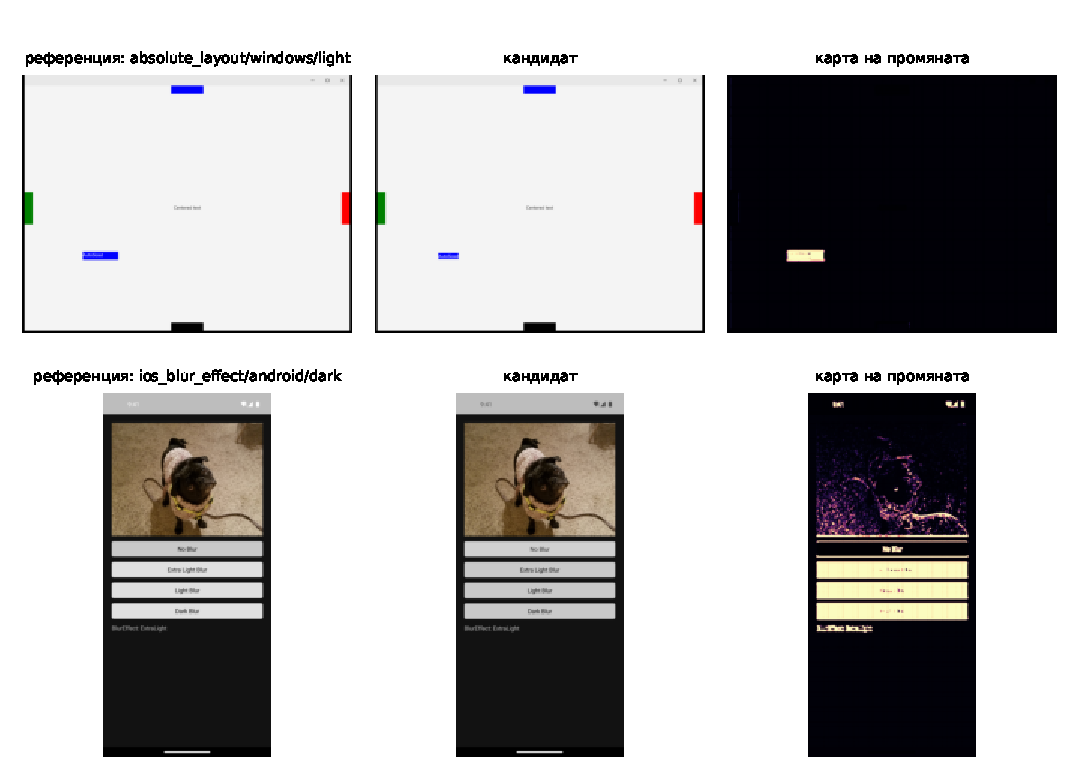
\includegraphics[width=\linewidth]{figures/heatmap.pdf}
\caption{Примери за картата на промяната на дообучената мрежа: референция, кандидат и вероятност за промяна. Негативната двойка (на втория ред) е активирана силно, което показва грешка на мрежата.}\label{fig:heat}
\end{figure}

Таблица~\ref{tab:gif} показва резултатите за GIF файловете. При само четири положителни двойки всички доверителни интервали са широки (от 0.16 до 0.91 за DTW), затова заключенията са предварителни. Оценката на мрежата върху кадри (0.725) е наситена за почти всички двойки и не може да се приеме за резултат.

\begin{table}[H]
\centering
\caption{GIF слоеве върху 34 двойки (4 DIFFERENT): AUC с доверителен интервал 95\% и балансирана точност при изпускане на по един етикет.}\label{tab:gif}
\begin{tabular}{lccc}
\hline
Слой & AUC (34) & 95\% ДИ & LOO точност \\
\hline
DTW~по~SSIM & 0.558 & [0.16, 0.91] & 0.558 \\
SSIM~на~първия~кадър & 0.438 & [0.07, 0.76] & 0.325 \\
хамфър~по~кадри & 0.558 & [0.16, 0.91] & 0.558 \\
CNN~по~кадри~(насищане) & 0.725 & [0.53, 0.90] & 0.675 \\
\hline
\end{tabular}

\end{table}

\subsection{Пример: оценка на GIF двойка}\label{sec:gifexample}
За да се види как работи оценката на GIF файловете, разглеждаме три двойки от набора с известни етикети. Всяка двойка минава през една и съща процедура: от всеки GIF се взимат кадрите, определя се област на движение (кадрите се сравняват с първия кадър и се взима обхващащият правоъгълник на пикселите с промяна над 0.04), в нея се построява матрица на разходите $C_{ij} = 1 - \text{SSIM}(A_i, B_j)$, а DTW намира най-евтиния монотонен път през $C$. Оценката е нормализираната цена на пътя, $s_{\text{DTW}} = \sum_{(i,j)\in P} C_{ij} / |P|$, а вердиктът се получава от прага $0.097$, избран върху всички GIF етикети (вж. раздел~\ref{sec:methods}).

Първата двойка \emph{android/swipe\_refresh\_dark} е DIFFERENT. Във втория GIF спинърът показва различно състояние на кадър 3 и DTW връща $s_{\text{DTW}} = 0.115$. Това е над прага, така че вердиктът е DIFFERENT, което съвпада с етикета.

Втората двойка \emph{android/selection\_synchronization\_dark} е SAME. Двата GIF файла се различават само по позицията на превъртане в по-късните кадри, но тази разлика е видима за DTW: $s_{\text{DTW}} = 0.178$, над прага. Вердиктът е DIFFERENT, което е грешно и обяснява четирите фалшиви положителни резултата в таблица~\ref{tab:gif}.

Третата двойка \emph{ios/switch\_light} е DIFFERENT, но $s_{\text{DTW}} = 0.0001$, под прага. Вердиктът е SAME, което е пропуснато положително. Слоят \emph{pixel\_frame0} (първият кадър) не помага тук, защото разликата се появява по-късно в анимацията.

\begin{figure}[H]
\centering
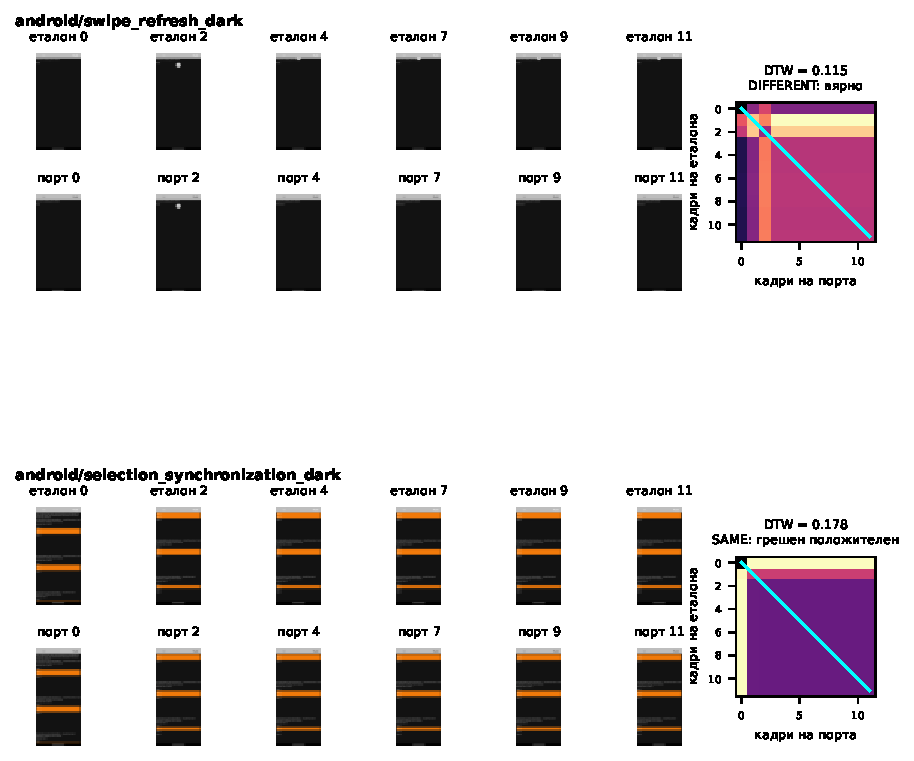
\includegraphics[width=\linewidth]{figures/gif_example.pdf}
\caption{Двете GIF двойки от раздел~\ref{sec:gifexample}. Всяка колона е стъпка по DTW пътя: горе е кадърът от еталона, долу – съответният кадър от порта (номерата са индексите на кадрите в GIF файла). Матрицата вдясно показва SSIM разходите (по-светло е по-скъпо) и DTW пътя в синьо.}\label{fig:gif}
\end{figure}

Тези три примера показват, че DTW е чувствителен към превъртане и не улавя разлики, които се появяват в кадри, различни от първия. Затова GIF резултатите в таблица~\ref{tab:gif} трябва да се четат като предварителни.

\section{Устойчивост към изместване}\label{sec:shift}
Основният практически въпрос е дали слоевете реагират на незначителни изменения на екрана. За да проверим това, изместваме кандидата хоризонтално с 0, 1, 2, 3 и 4 пиксела (с повторено гранично пиксели) и пресмятаме всички статични слоеве отново. Прагът на всеки слой е фиксиран при 0 пиксела, така че при по-голямо изместване се вижда как се променя поведението му.

Таблица~\ref{tab:shift} показва два показателя за всеки слой и изместване. ЛА (лъжлива аларма) е делът на SAME двойките, които се маркират като DIFFERENT; колкото по-нисък, толкова по-добре. ОД (откриване) е делът на DIFFERENT двойките, които се маркират като DIFFERENT; колкото по-висок, толкова по-добре. Прагът е избран върху 0-пикселовите етикети и се използва непроменен за всички измествания, което е оптимистична оценка за устойчивостта, тъй като прагът е настроен на същите двойки.

\begin{table}[H]
\centering
\caption{Устойчивост на слоевете към хоризонтално изместване на кандидата. ЛА – дял на SAME двойките, маркирани като DIFFERENT (по-ниско е по-добре); ОД – дял на DIFFERENT двойките, маркирани като DIFFERENT (по-високо е по-добре).}\label{tab:shift}
\scriptsize
\begin{tabular}{lcccccccccc}
\hline
Метод & \multicolumn{2}{c}{0 px} & \multicolumn{2}{c}{1 px} & \multicolumn{2}{c}{2 px} & \multicolumn{2}{c}{3 px} & \multicolumn{2}{c}{4 px} \\
 & ЛА & ОД & ЛА & ОД & ЛА & ОД & ЛА & ОД & ЛА & ОД \\
\hline
SSIM по плочки (базова) & 0.23 & 0.49 & 0.30 & 0.55 & 0.59 & 0.66 & 0.69 & 0.79 & 0.82 & 0.85 \\
GMSD & 0.66 & 0.98 & 1.00 & 1.00 & 1.00 & 1.00 & 1.00 & 1.00 & 1.00 & 1.00 \\
Chamfer по контури & 0.62 & 0.94 & 1.00 & 1.00 & 1.00 & 1.00 & 1.00 & 1.00 & 1.00 & 1.00 \\
Цветови хистограми & 0.48 & 0.68 & 0.49 & 0.68 & 0.48 & 0.68 & 0.49 & 0.68 & 0.49 & 0.68 \\
LBP текстура & 0.34 & 0.77 & 0.36 & 0.77 & 0.44 & 0.77 & 0.43 & 0.74 & 0.44 & 0.79 \\
ORB + RANSAC & 0.43 & 0.68 & 0.90 & 1.00 & 0.97 & 1.00 & 0.98 & 1.00 & 0.98 & 1.00 \\
Сегменти (k-means) & 1.00 & 1.00 & 1.00 & 1.00 & 1.00 & 1.00 & 1.00 & 1.00 & 1.00 & 1.00 \\
ResNet-18 плочки (max) & 0.43 & 0.83 & 0.43 & 0.81 & 0.52 & 0.85 & 0.52 & 0.85 & 0.52 & 0.83 \\
ResNet-18 плочки (топ-5) & 0.23 & 0.68 & 0.23 & 0.70 & 0.26 & 0.66 & 0.33 & 0.68 & 0.33 & 0.70 \\
DINOv2 плочки (max) & 0.39 & 0.77 & 0.39 & 0.81 & 0.52 & 0.81 & 0.57 & 0.85 & 0.59 & 0.85 \\
DINOv2 плочки (топ-5) & 0.21 & 0.62 & 0.23 & 0.64 & 0.31 & 0.66 & 0.39 & 0.70 & 0.41 & 0.74 \\
\hline
\end{tabular}

\end{table}

Пикселният SSIM се влошава бързо: ЛА нараства от 0.23 при 0 пиксела до 0.82 при 4 пиксела. Това е точно поведението, което не искаме за желан интерфейс, който не се променя. LBP текстурата се влошава по-бавно (ЛА от 0.34 до 0.44), а ResNet-18 с топ-5 плочки (от 0.23 до 0.33) и DINOv2 с топ-5 плочки (от 0.21 до 0.41) са по-устойчиви. ORB с RANSAC изненадващо е най-чувствителен: ЛА скача от 0.43 на 0.90 при 1 пиксел, въпреки че хомографията трябва да покрива изместването. Вероятно причината е, че дескрипторите на ORB се променят при целочислено изместване на пикселната решетка, което намалява числото на съвпадения, преминали теста на отношението, а не RANSAC. Това не сме проверили експериментално.

GMSD, хамфър и сегментацията маркират почти всичко като DIFFERENT още при 1 пиксел, защото праговете им са фиксирани при 0 пиксела и са твърде ниски за изместеното изображение. Сегментацията има праг 0.0 и маркира всичко; това е вырожден праг, който отразява слабата й връзка с етикетите. Цветовите хистограми са устойчиви на изместване (ЛА 0.48–0.49), но пропускат част от DIFFERENT двойките (ОД 0.68).

\section{Дискусия и заключение}\label{sec:discussion}

От резултатите следват три извода. Първо, върху всички двойки стекингът и дълбоките плочкови признаци дават високи AUC, но тази оценка е завишена от съгласуваните двойки, които са лесни за AI прегледите. Второ, върху спорните двойки, проверени от човек, най-добрите слоеве са GMSD и хамфър разстоянието по контури, а дълбоките признаци са близо до случайното. Трето, пикселният SSIM и цветовите хистограми са обърнати върху спорните двойки и не могат да се използват като самостоятелен критерий. Ограниченията са няколко. Консенсусните етикети не са човешки проверени и може да повтарят грешки на двата AI прегледа, затова най-надеждната оценка е върху спорните 204 двойки, където човек е решил. Спорните двойки са избрани от разлика между прегледите, така че са по-трудни от средната двойка. GIF файловете са само 34, а MINOR се третира като SAME. Не сме възпроизвели предишния резултат 0.91, защото признаците му не са в хранилището.

Следващите стъпки са: да се събират етикети върху реални промени в продукцията спрямо дизайна във Figma, да се тестват и други трансформации (мащаб, промяна на шрифт, леко преоцветяване), да се калибрират праговете върху отделна извадка, да се подравняват GIF кадрите по време преди съпоставяне, и да се провери дали ORB е чувствителен към целочислено изместване.

\begin{thebibliography}{99}
\bibitem{wang2004} Wang Z., Bovik A.~C., Sheikh H.~R., Simoncelli E.~P. Image quality assessment: from error visibility to structural similarity. \emph{IEEE Transactions on Image Processing}, 13(4), 600--612, 2004.
\bibitem{xue2014} Xue W., Zhang L., Mou X., Bovik A.~C. Gradient magnitude similarity deviation: a highly efficient perceptual image quality index. \emph{IEEE Transactions on Image Processing}, 23(2), 684--695, 2014.
\bibitem{canny1986} Canny J. A computational approach to edge detection. \emph{IEEE Transactions on Pattern Analysis and Machine Intelligence}, 8(6), 679--698, 1986.
\bibitem{borgefors1988} Borgefors G. Hierarchical chamfer matching: a parametric edge matching algorithm. \emph{IEEE Transactions on Pattern Analysis and Machine Intelligence}, 10(6), 849--865, 1988.
\bibitem{ojala2002} Ojala T., Pietikäinen M., Mäenpää T. Multiresolution gray-scale and rotation invariant texture classification with local binary patterns. \emph{IEEE Transactions on Pattern Analysis and Machine Intelligence}, 24(7), 971--987, 2002.
\bibitem{rublee2011} Rublee E., Rabaud V., Konolige K., Bradski G. ORB: an efficient alternative to SIFT or SURF. In: \emph{Proc. ICCV}, 2564--2571, 2011.
\bibitem{fischler1981} Fischler M.~A., Bolles R.~C. Random sample consensus: a paradigm for model fitting with applications to image analysis and automated cartography. \emph{Communications of the ACM}, 24(6), 381--395, 1981.
\bibitem{he2016} He K., Zhang X., Ren S., Sun J. Deep residual learning for image recognition. In: \emph{Proc. CVPR}, 770--778, 2016.
\bibitem{oquab2024} Oquab M. et al. DINOv2: learning robust visual features without supervision. \emph{Transactions on Machine Learning Research}, 2024.
\bibitem{daudt2018} Daudt R.~C., Le Saux B., Boulch A. Fully convolutional siamese networks for change detection. In: \emph{Proc. ICIP}, 4063--4067, 2018.
\bibitem{ronneberger2015} Ronneberger O., Fischer P., Brox T. U-Net: convolutional networks for biomedical image segmentation. In: \emph{Proc. MICCAI}, 234--241, 2015.
\bibitem{kingma2015} Kingma D.~P., Ba J. Adam: a method for stochastic optimization. In: \emph{Proc. ICLR}, 2015.
\bibitem{berndt1994} Berndt D.~J., Clifford J. Using dynamic time warping to find patterns in time series. In: \emph{Proc. AAAI Workshop on Knowledge Discovery in Databases}, 359--370, 1994.
\bibitem{hanley1982} Hanley J.~A., McNeil B.~J. The meaning and use of the area under a receiver operating characteristic (ROC) curve. \emph{Radiology}, 143(1), 29--36, 1982.
\bibitem{efron1993} Efron B., Tibshirani R.~J. \emph{An Introduction to the Bootstrap}. Chapman \& Hall, 1993.
\end{thebibliography}

\end{document}
